\section{Structures}

\begin{figure}[h!]
    \centering
    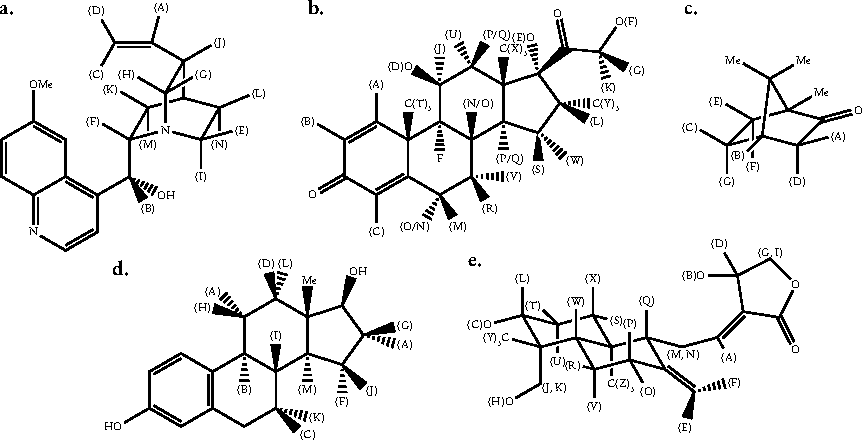
\includegraphics{structures/structures_final.pdf}
    \caption[
        The molecular structures of species giving rise to the experimental
        \acs{NMR} datasets considered in this work.
    ]{
        The molecular structures of species giving rise to the experimental
        \acs{NMR} datasets considered in this work.
        \textbf{a.} Quinine,
        \textbf{b.} Dexamethasone,
        \textbf{c.} Camphor,
        \textbf{d.} 17\textbeta-estradiol,
        \textbf{e.} Andrographolide.
        Proton environments giving rise to signals which are considered in this
        work are denoted with bracketed alphabetical characters. Non-bracketed
        alphabetical characters denote chemical symbols. \ch{Me} denotes the methyl
        group, equivalent to \ch{CH3}.
        \note{
            TODO: check assignments (esp. estradiol). If more structures need
            adding, edit the ChemDraw file on Chive called
            \path{simon_stuff/thesis_structures.cdxml}. Use EB-Garamond for
            atom labels. One a structure is made, scale to 75\% of original
            size, and set font to 7pt. Then in inkscape, rescale this by
            multiplying by 0.8.
        }
    }
    \label{fig:structures}
\end{figure}
